\section{Approach}

\subsection{Designing Recovery Scenarios}
To test the DFR tools' compliance with the standards, we designed a variety of scenarios in which a tool might have to recover a deleted file. We started with the simplest possible case: a filesystem containing just one deleted file. This case is ideal and trivial, but by adding more files, we can create far more complex scenarios.

% Fragmentation and Overwriting are the two things that can complicate file recovery 
The NIST standards limit the scope of testing to situations in which files were ``created and deleted in a process similar to how an end-user would create and delete files,'' and  exclude ``files and file system metadata that is specifically corrupted, modified, or otherwise manipulated to appear deleted.'' %TODO cite quotes from the standards
Within these constraints, there are two factors which can significantly complicate the file recovery process: fragmentation, and overwriting. %TODO make sure these are defined elsewhere, if not, define them here
% Make different varieties of Fragmentation and overwriting, and combinations
These factors are thus the focus of our test scenarios, with all cases besides the first involving either fragmented files, overwritten files, or a combination of both.

% Fragmentation is trivial in NTFS so less interesting
% Explanation of each test case
% Show a few figures for interesting test cases

\subsection{Creating Test Images}
% Step by step process
All test filesystems were created in partitions on a 32 GB flash drive. For each test case, the first step is to entirely write over the partition with zeros. This ensures all cases start from identical, reproduceable conditions. A new filesystem is written to the partition, then new files are written to the filesystem and deleted. The files used are simple text files containing one letter repeated (e.g. ``aa1M'' is 1 MiB of the letter 'a'). Files are written to the test filesystem by simply copying them from another drive. In some cases we also append data to a file in the test filesystem. Once the test filesystem matches the intended scenario, a read-only image of the partition is created. All tests are performed on these images rather than the original drive.

% Caching problem
It is important to consider when creating test images that the low-level behavior of file operations is not always obvious. For example, when writing a file, there is no guarantee the file's data will be immediately written to the disk. The operating system may cache the operation and wait until the optimal time to perform the write, in order to maximize system performance. We observed this early on, as writing a file and subsequently deleting it would always result in the file's metadata being written, but often left no evidence of the file's data having ever existed. This behavior is obviously undesireable because it leaves nothing meaningful to be recovered. We resolved this by calling the ``sync'' system call, which causes any such cached data to be immediately written to the disk, in between file writes and deletions. Unmounting the filesystem has a similar effect.

% Learning and using the allocation algorithms
Another type of low-level behavior relevant to the image creation process is the allocation algorithm. The operating system must have some kind of algorithm to decide where in the data area new files should be written. Common allocation algorithms include ``first available,'' ``next available,'' and ``best fit.'' %TODO cite
Learning and understanding whatever algorithm the OS uses is very helpful for forcing a specific arrangement of files. We observed that when writing to a FAT filesystem, Linux uses a ``next available'' algorithm. After the filesystem is mounted, the first write will start at the first free space in the data area. The next file will be written starting from the first free space after the previous file.
Meanwhile, when writing to an NTFS filesystem, Windows 10 appears to use a ``best fit'' algorithm. In this case, Windows tries to find the smallest space in which the file can fit without being fragmented, and write it there.

% Directory entries problem

\subsection{Recovering Files}


\subsection{Results}
% Figures with results
\begin{figure}[h!]
    \centering

    \begin{subfigure}{0.3\linewidth}
        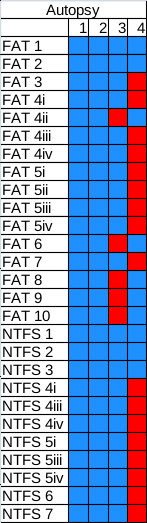
\includegraphics[width=\linewidth]{fig/autopsy_results.png}
        \subcaption{Autopsy}
    \end{subfigure}
    ~
    \begin{subfigure}{0.3\linewidth}
        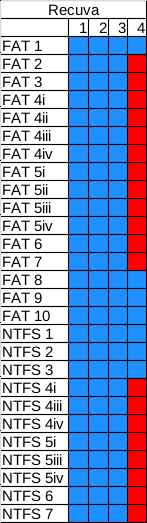
\includegraphics[width=\linewidth]{fig/recuva_results.png}
        \subcaption{Recuva}
    \end{subfigure}
    ~
    \begin{subfigure}{0.3\linewidth}
        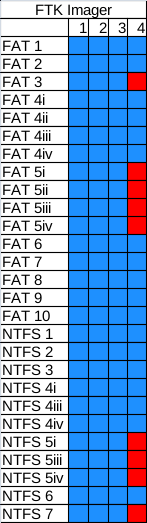
\includegraphics[width=\linewidth]{fig/ftk_results.png}
        \subcaption{FTK}
    \end{subfigure}
    
    
    \begin{subfigure}{0.3\linewidth}
        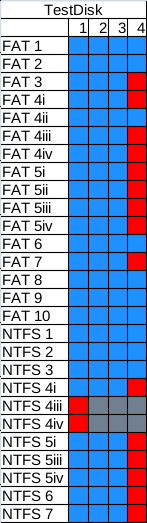
\includegraphics[width=\linewidth]{fig/testdisk_results.png}
        \subcaption{TestDisk}
    \end{subfigure}
    ~
    \begin{subfigure}{0.3\linewidth}
        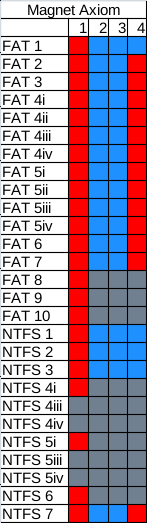
\includegraphics[width=\linewidth]{fig/axiom_results.png}
        \subcaption{Magnet Axiom}
    \end{subfigure}
    
    \caption{Test Results}
    \label{fig:results}
\end{figure}

% Explain Magnet Axiom filenames issue
